\problemset{Теория вероятностей и математическая статистика}
\problemset{Индивидуальное домашнее задание №4}

% Команда ниже задает "название" или слово, которое будет
% отображаться вместо proof или "доказательство"
% поскольку у нас в ИДЗ задачи - то нужно слово "Решение"
\renewcommand*{\proofname}{Решение}
Матрица вероятностей перехода однородной цепи Маркова имеет вид
\[
P = \frac{1}{10}\begin{pmatrix}
    2 & 0 & 0 & 0 & 2 & 4 & 2 & 0 \\
    0 & 4 & 0 & 6 & 0 & 0 & 0 & 0 \\
    3 & 0 & 4 & 0 & 2 & 0 & 1 & 0 \\
    0 & 5 & 0 & 5 & 0 & 0 & 0 & 0 \\
    1 & 0 & 4 & 0 & 3 & 2 & 0 & 0 \\
    2 & 0 & 0 & 0 & 2 & 5 & 1 & 0 \\
    4 & 0 & 3 & 0 & 0 & 3 & 0 & 0 \\
    0 & 3 & 0 & 1 & 0 & 3 & 3 & 0 \\
\end{pmatrix}
\]

%%%%%%%%%%%%%% ЗАДАНИЕ №1 %%%%%%%%%%%%%%
%% Условие задания №1
\begin{problem}
Определить матрицу вероятностей перехода за два шага.
\end{problem}

%% Решение задания №1
\begin{proof}
\[
P^{(2)} = P^2 = \frac{1}{100}\begin{pmatrix}
    22 & 0  & 14 & 0  & 18 & 38 & 8  & 0 \\
    0  & 46 & 0  & 54 & 0  & 0  & 0  & 0 \\
    24 & 0  & 27 & 0  & 20 & 19 & 10 & 0 \\
    0  & 45 & 0  & 55 & 0  & 0  & 0  & 0 \\
    21 & 0  & 28 & 0  & 23 & 20 & 8  & 0 \\
    20 & 0  & 11 & 0  & 20 & 40 & 9  & 0 \\
    23 & 0  & 12 & 0  & 20 & 31 & 14 & 0 \\
    18 & 17 & 9  & 23 & 6  & 24 & 3  & 0
\end{pmatrix}
\]
\end{proof}

%%%%%%%%%%%%%% ЗАДАНИЕ №2 %%%%%%%%%%%%%%
%% Условие задания №2
\begin{problem}
Выделить классы сообщающихся состояний.
\end{problem}

%% Решение задания №2
\begin{proof}
Нарисуем граф (рис.1). На рисунке все веса делить на 10.\\
\begin{figure}[h!]
    \centering
    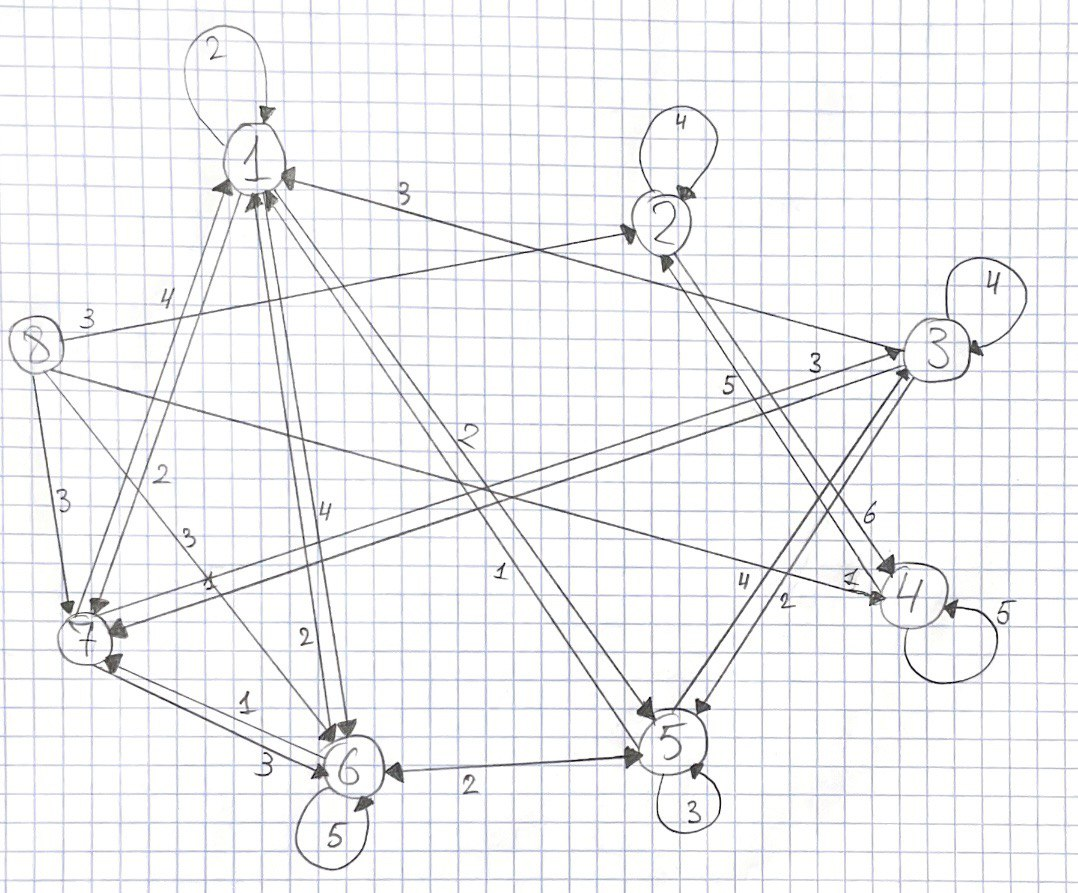
\includegraphics[width=0.5\linewidth]{1.jpeg}
    \caption{}
    \label{fig:enter-label}
\end{figure}
Смотрим, анализируем и получаем следующие классы сообщающихся состояний:\\
$E_0 = $ {8}\\
$E_1 = $ {1, 3, 5, 6, 7}\\
$E_2 = $ {2, 4}\\
\end{proof}

%%%%%%%%%%%%%% ЗАДАНИЕ №3 %%%%%%%%%%%%%%
%% Условие задания №3
\begin{problem}
Есть ли невозвратные состояния?
\end{problem}

%% Решение задания №3
\begin{proof}
Да. Состояние 8. В него невозможно вернуться, покинув его. Это невозвратное (или несущественное) состояние.
\end{proof}

%%%%%%%%%%%%%% ЗАДАНИЕ №4 %%%%%%%%%%%%%%
%% Условие задания №4
\begin{problem}
Найти период в каждом из классов.
\end{problem}

%% Решение задания №4
\begin{proof}
Матрица класса 1:
\[
P_1 = \frac{1}{10}\begin{pmatrix}
    2 & 0 & 2 & 4 & 2 \\
    3 & 4 & 2 & 0 & 1 \\
    1 & 4 & 3 & 2 & 0 \\
    2 & 0 & 2 & 5 & 1 \\
    4 & 3 & 0 & 3 & 0
\end{pmatrix}
\]
m = 1 для i = {1, 3, 5, 6}.\\
\[
P_1^2 = \frac{1}{100}\begin{pmatrix}
    14 & 8  & 18 & 32 & 4 \\
    24 & 27 & 20 & 19 & 4 \\
    21 & 28 & 23 & 20 & 6 \\
    20 & 11 & 20 & 40 & 5 \\
    23 & 12 & 20 & 31 & 6
\end{pmatrix}
\]
m = 2 для i = 7.\\
НОД(1, 2) = 1, то есть период класса 1 равен 1, он апериодичный\\
Матрица класса 2:
\[
P_1 = \frac{1}{10}\begin{pmatrix}
    4 & 6 \\
    5 & 5
\end{pmatrix}
\]
Тут всего один m = 1 для i = {2, 4}, значит что период класса 2 равен 1, он апериодичный.
\end{proof}

%%%%%%%%%%%%%% ЗАДАНИЕ №5 %%%%%%%%%%%%%%
%% Условие задания №5
\begin{problem}
Вычислить финальные вероятности в каждом классе.
\end{problem}

%% Решение задания №5
\begin{proof}
Для класса 1:
\begin{gather*}
    x = (p_1, p_3, p_5, p_6, p_7)\\
    \begin{cases}
        (P_1^T - I)x^T = 0 \\
        \sum_i p_i = 1
    \end{cases} \Rightarrow \\
    \begin{cases}
        (10P_1^T - 10I)x^T = 0 \\
        \sum_i p_i = 1
    \end{cases}
\end{gather*}
В первом уравнении системы получили систему однородных уравнений. Она имеет матрицу:
\[
\begin{pmatrix}
    -8 & 3 & 1 & 2 & 4 \\
    0 & -6 & 4 & 0 & 3 \\
    2 & 2 & -7 & 2 & 0 \\
    4 & 0 & 2 & -5 & 3 \\
    2 & 1 & 0 & 1 & -10 \\
\end{pmatrix}
\]
Решаем систему и получаем ответ $x = (\frac{1229}{524}p_7, \frac{513}{262}p_7, \frac{573}{262}p_7, \frac{439}{131}p_7, p_7)$. Воспользуемся вторым условием $\sum_i p_i = 1$ и получим:\\
\begin{gather*}
    p_1 = \frac{1229}{5681}\approx 0.2163\\
    p_3 = \frac{54}{299}\approx 0.1806\\
    p_5 = \frac{1146}{5681}\approx 0.2017\\
    p_6 = \frac{1756}{5681}\approx 0.3091\\
    p_7 = \frac{524}{5681}\approx 0.0922
\end{gather*}

Для класса 2:
\begin{gather*}
    x = (p_2, p_4)\\
    \begin{cases}
        (P_2^T - I)x^T = 0 \\
        \sum_i p_i = 1
    \end{cases} \Rightarrow \\
    \begin{cases}
        (10P_2^T - 10I)x^T = 0 \\
        \sum_i p_i = 1
    \end{cases}
\end{gather*}
Матрица однордной системы:
\[
\begin{pmatrix}
    -6 & 5 \\
     6 & -5
\end{pmatrix}
\]
Её решение: $x = (\frac{5}{6}p_4, p_4)$. Воспользуемся вторым условием и получим:\\
\begin{gather*}
    p_2 = \frac{5}{11}\approx 0.4545\\
    p_4 = \frac{6}{11}\approx 0.5454\\
\end{gather*}
Поскольку состояние 8 - несущественное, $p_8 = 0$.
\end{proof}

Задания 6 и 7: https://github.com/timohahaa/PT-MS/blob/main/sim.ipynb